\documentclass{article}

\usepackage{authblk}
\usepackage{graphicx}
\usepackage{float}
\usepackage{tabu}
\usepackage{multirow}
\usepackage{xcolor}

\title{Supplement: Data exploration, quality control and statistical
  analysis of ChIP-exo experiments}
\date{}

\newcommand{\beginsupplement}{%
        \setcounter{table}{0}
        \renewcommand{\thetable}{S\arabic{table}}%
        \setcounter{figure}{0}
        \renewcommand{\thefigure}{S\arabic{figure}}%
     }


\author[1]{Rene Welch}
\author[6]{Dongjun Chung}
\author[3]{Irene Ong}
\author[3,4]{Jeffrey Grass}
\author[3,4,5]{Robert Landick}
\author[1,2]{S\"und\"uz Kele\c{s}}


\affil[1]{Department of Statistics, University of Wisconsin Madison}
\affil[2]{Department of Biostatistics and Medical Informatics,
  University of Wisconsin Madison}
\affil[3]{Great Lakes Bioenergy Research Center, University of Wisconsin Madison}
\affil[4]{Department of Biochemistry, University of Wisconsin Madison}
\affil[5]{Department of Bacteriology, University of Wisconsin Madison}
\affil[6]{Department of Public Health Sciences, Medical University of South Carolina}

\newcommand{\sig}{\sigma^{70}}

\newcommand{\pname}[1]{\texttt{ChIPexoQual}}
\newcommand{\SK}[1]{\textcolor{red}{SK: #1}}
\newcommand{\RW}[1]{\textcolor{blue}{RW: #1}}


\begin{document}

\maketitle

\beginsupplement

\tableofcontents

\newpage

\section{Comparison of ChIP-exo with ChIP-Seq data.}

\begin{figure}[H]
  \centering
  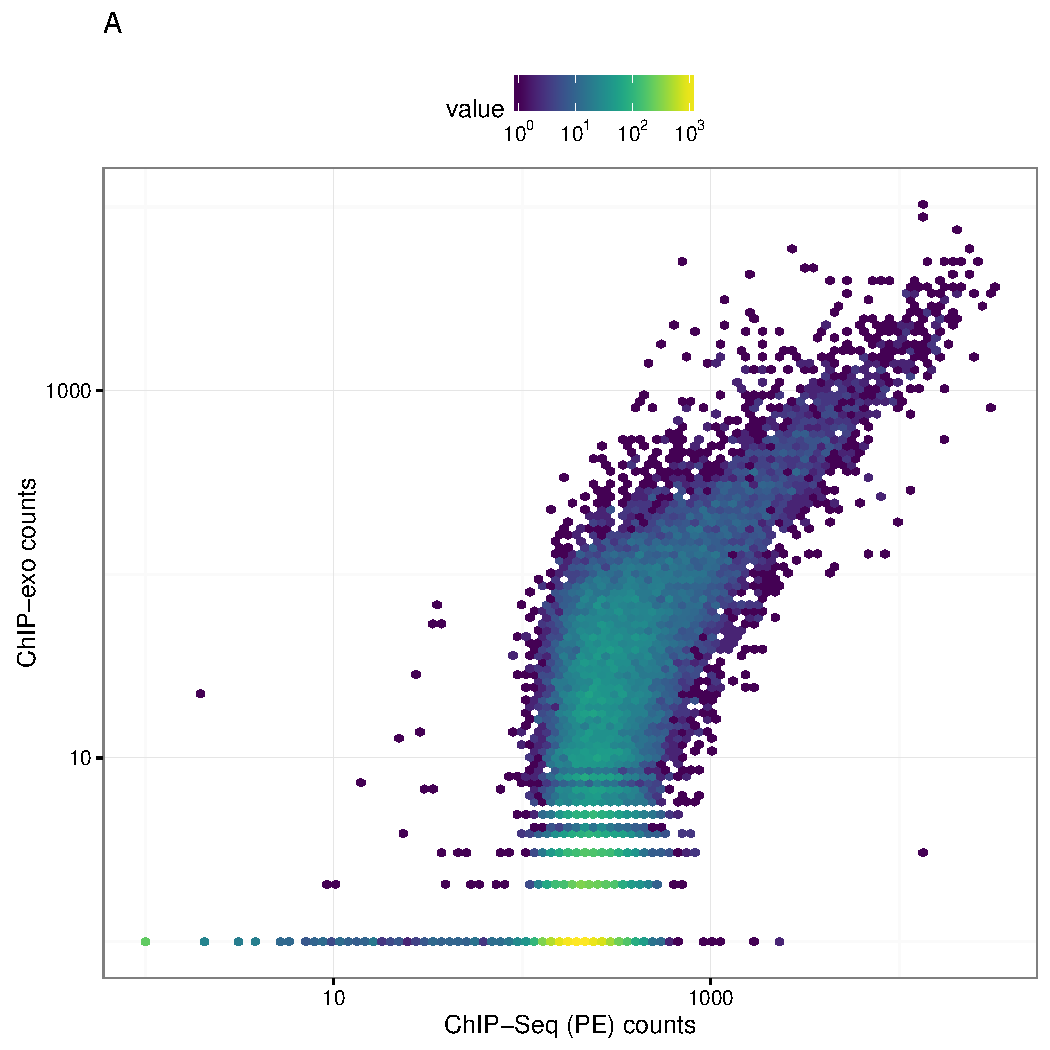
\includegraphics[width =
  .35\textwidth,page = 1]{figures/supplement/ChIPSeq_comp/sig70_rif_count_comparison.pdf}
  \includegraphics[width =
  .35\textwidth,page = 2]{figures/supplement/ChIPSeq_comp/sig70_rif_count_comparison.pdf}
  \includegraphics[width =
  .35\textwidth,page = 3]{figures/supplement/ChIPSeq_comp/sig70_rif_count_comparison.pdf}
  \includegraphics[width =
  .35\textwidth,page = 4]{figures/supplement/ChIPSeq_comp/sig70_rif_count_comparison.pdf}
  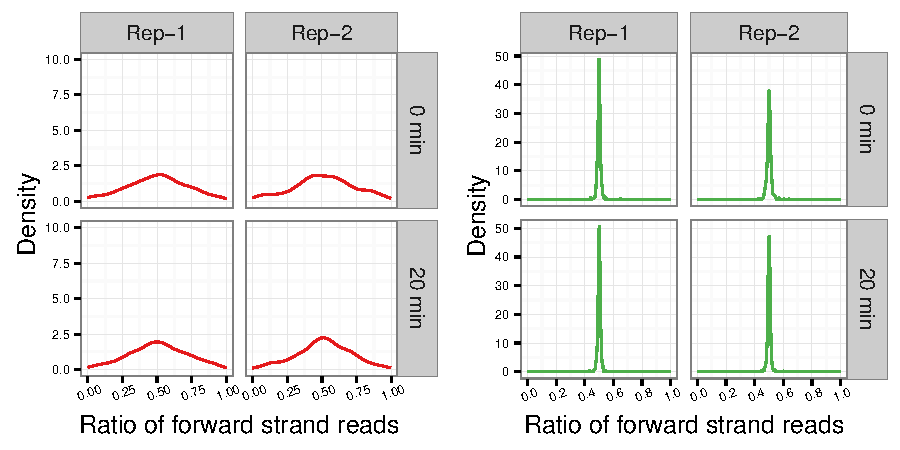
\includegraphics[width =
  .9\textwidth]{figures/supplement/ChIPSeq_comp/Sig70_strand_imbalance_rif.pdf}
  \caption{Hexbin plots of PE ChIP-Seq bin counts vs. ChIP-exo bin
    counts for $\sigma^{70}$ second biosample: A) E2-1, B) E2-2 C)
    E2-3 and D) E2-4 samples. E) Forward Strand Ratio densities for SE
    ChIP-Seq and ChIP-exo peaks for $\sigma^{70}$, S2 and E2 groups
    respectively.}
  \label{sfig:comp1}
\end{figure}


\begin{figure}[H]
  \centering
  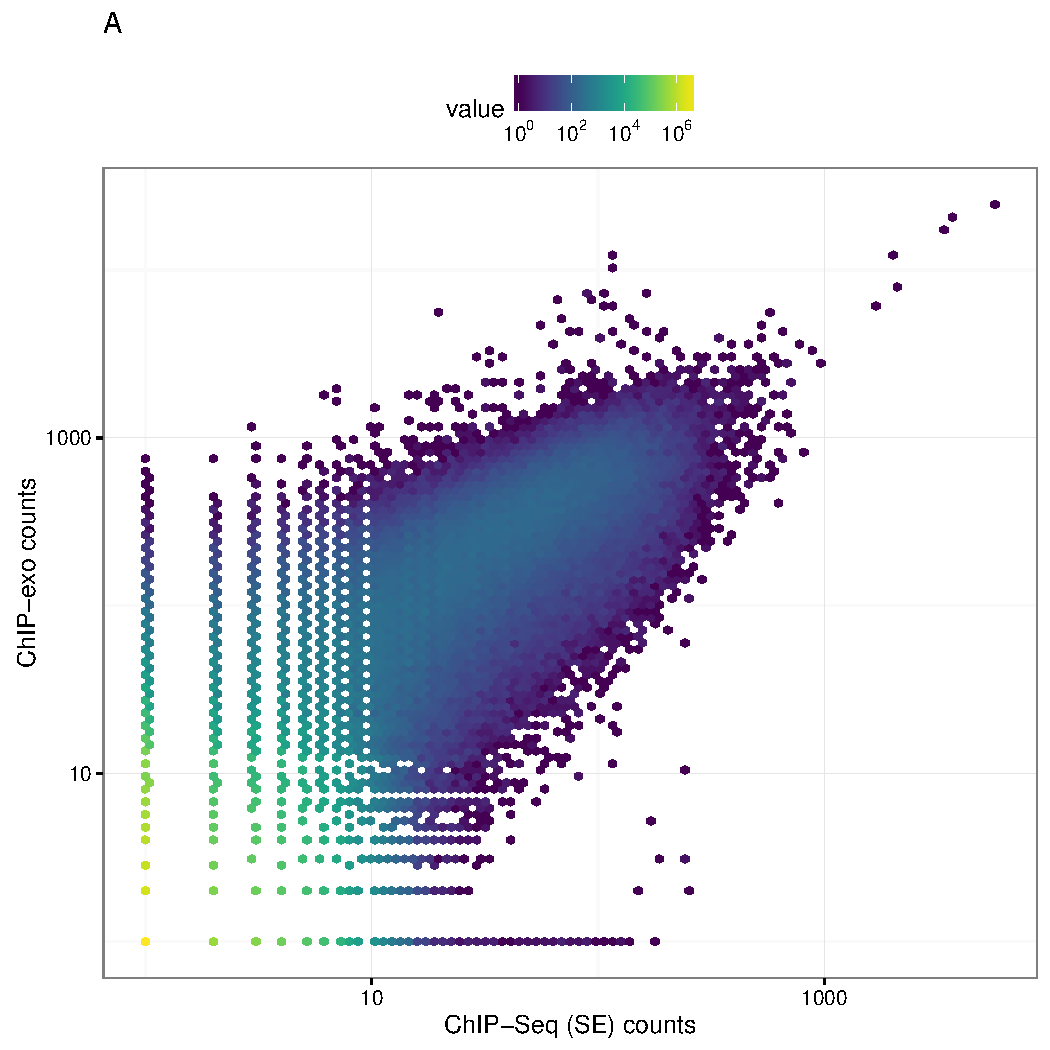
\includegraphics[width = .35\textwidth,page =
  1]{figures/supplement/ChIPSeq_comp/pugh_CTCF_human_bin_comp.pdf}
  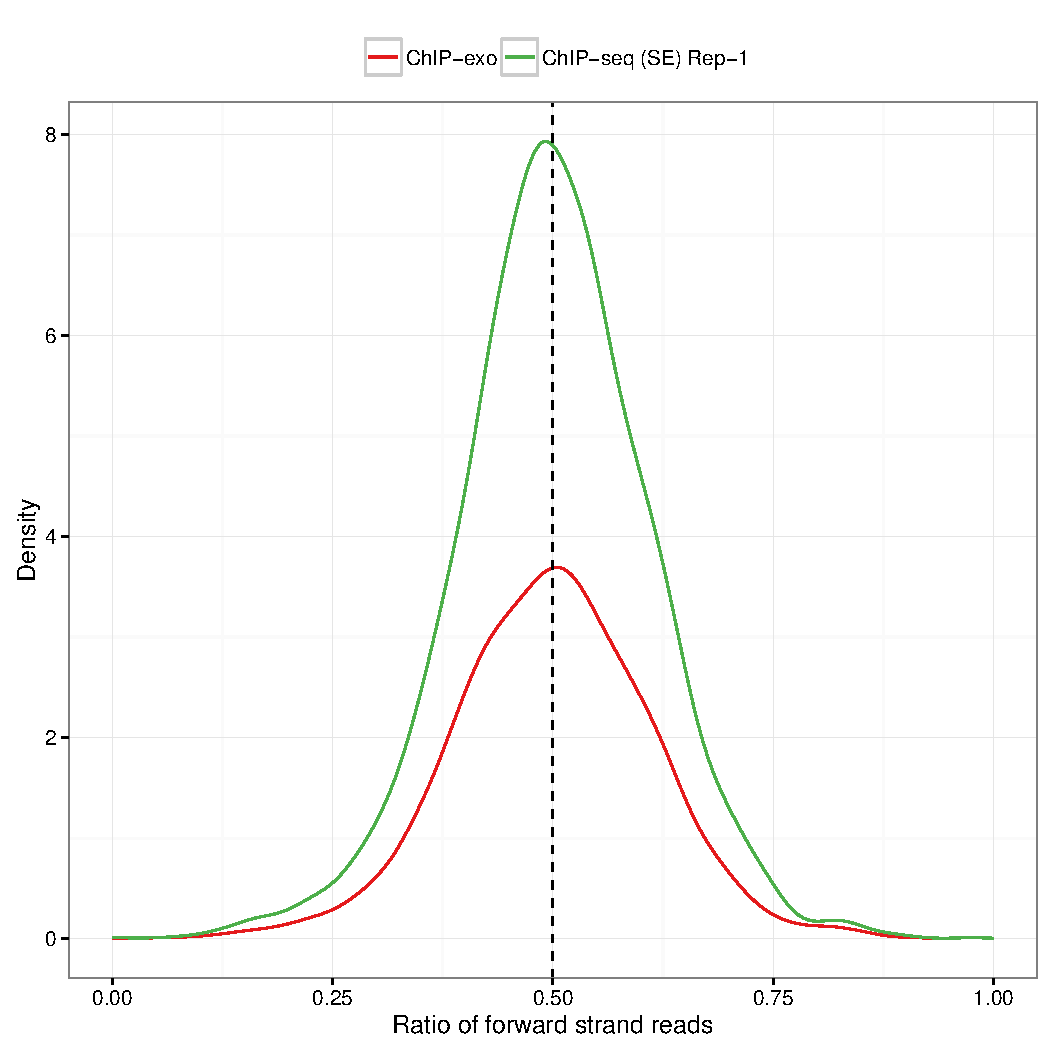
\includegraphics[width = .35\textwidth,page =
  1]{figures/supplement/ChIPSeq_comp/CTCF_imbalance.pdf}
  \includegraphics[width = .35\textwidth,page =
  2]{figures/supplement/ChIPSeq_comp/pugh_CTCF_human_bin_comp.pdf}
  \includegraphics[width = .35\textwidth,page =
  2]{figures/supplement/ChIPSeq_comp/CTCF_imbalance.pdf}
  \caption{Hexbin plot comparing A) Rep-1 and B) Rep-2 ENCODE SE
    ChIP-seq bin counts vs. Pugh ChIP-exo bin counts for CTCF in HeLa
    cell. C) Rep-1 and D) Rep-2 ChIP-seq compared against ChIP-exo
    Forward Strand Ratio densities.}
  \label{sfig:comp2}
\end{figure}


\begin{figure}[H]
  \centering
  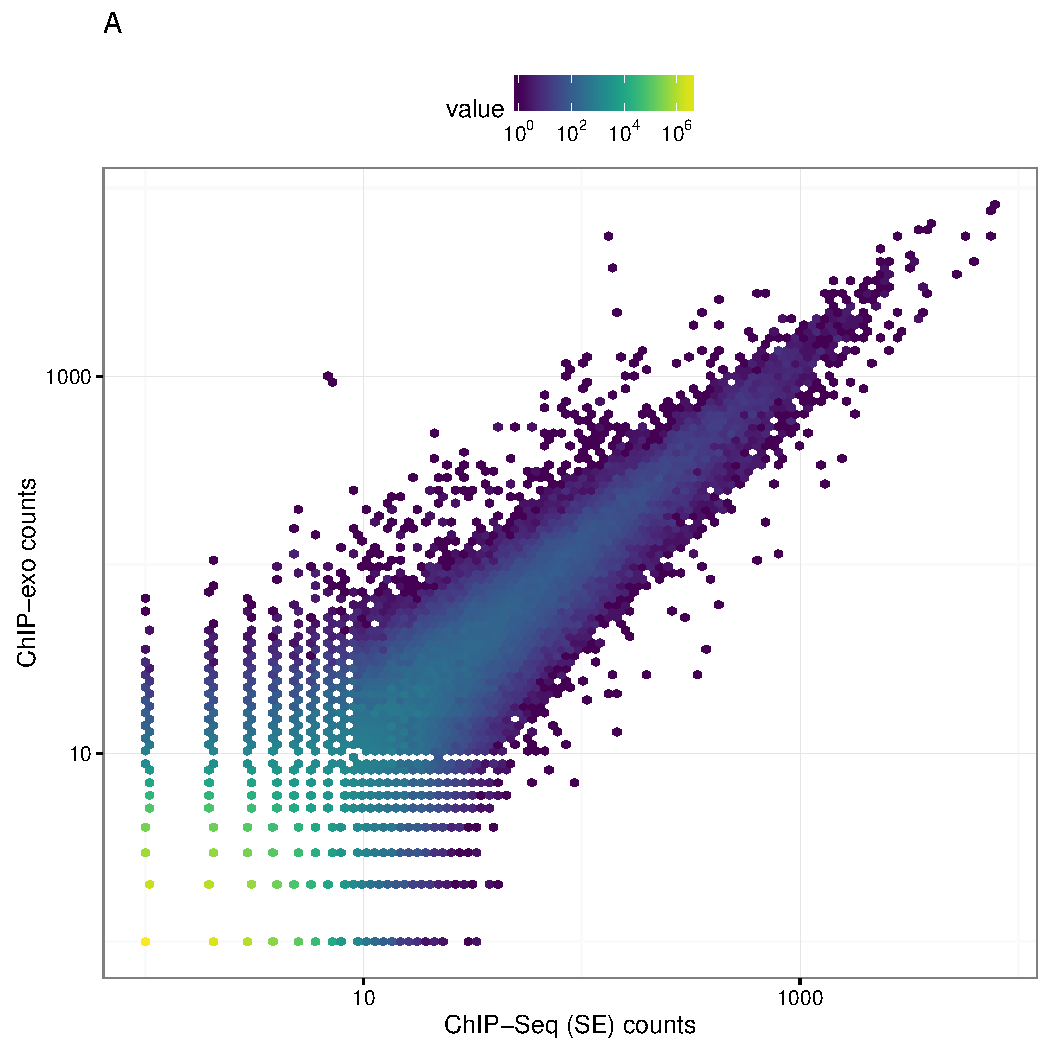
\includegraphics[width =.35\textwidth,page =
  1]{figures/supplement/ChIPSeq_comp/carroll_ER_human_bin_comp.pdf}
  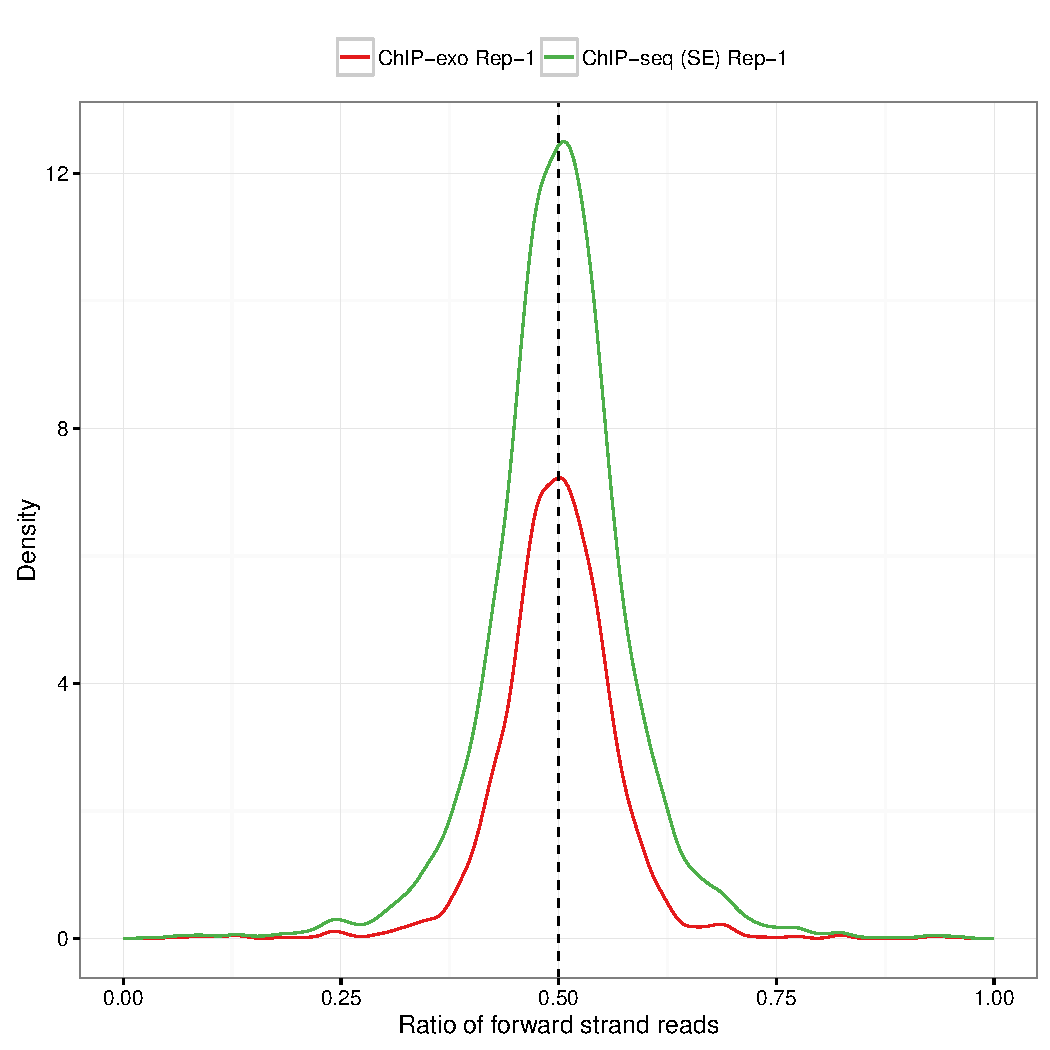
\includegraphics[width = .35\textwidth,page =
  1]{figures/supplement/ChIPSeq_comp/ER_imbalance.pdf}
  \includegraphics[width =.35\textwidth,page =
  2]{figures/supplement/ChIPSeq_comp/carroll_ER_human_bin_comp.pdf}
  \includegraphics[width = .35\textwidth,page =
  2]{figures/supplement/ChIPSeq_comp/ER_imbalance.pdf}
  \includegraphics[width =.35\textwidth,page =
  3]{figures/supplement/ChIPSeq_comp/carroll_ER_human_bin_comp.pdf}
  \includegraphics[width = .35\textwidth,page =
  3]{figures/supplement/ChIPSeq_comp/ER_imbalance.pdf}
  \caption{Hexbin plots comparing SE ChIP-Seq bin counts vs. ChIP-exo
    bin counts for ER in human MCF-7 cell lines. }
  \label{sfig:comp3}
\end{figure}

% \RW{ we also have data to add comparison of ChIP-exo vs ChIP-Seq TBP
%   in K562 cell lines, I am not eager to include those because 1) the
%   chip-exo data is of low quality, 2)}


\newpage

\section{SCC curves for ChIP-exo and ChIP-nexus data.}

\begin{figure}[H]
  \centering
  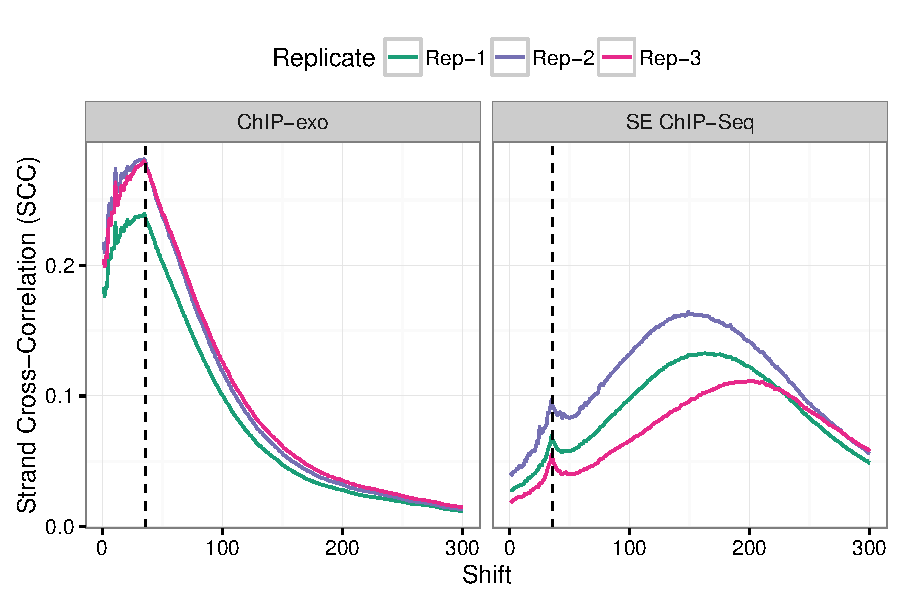
\includegraphics[width =
  .7\textwidth]{figures/supplement/SCC/Carroll_human_SCC.pdf}
  \caption{Comparison of ChIP-exo vs. ChIP-Seq SCC curves for ER factor in
    human MCF-7 cell lines. }
\label{sfig:scc1}
\end{figure}

\begin{figure}[H]
  \centering
  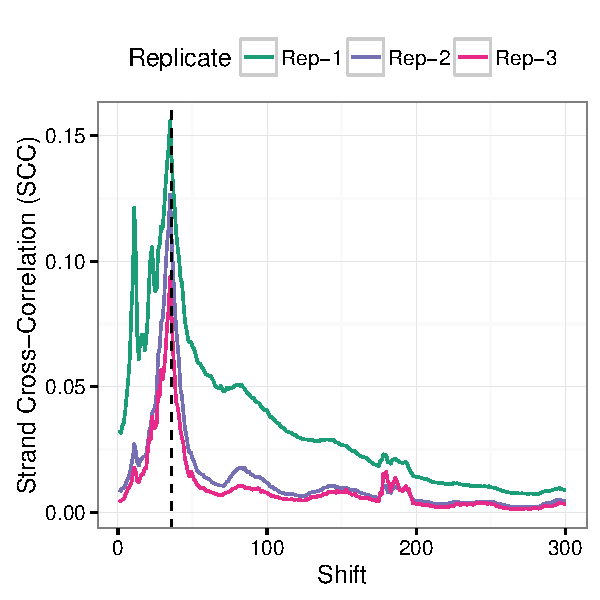
\includegraphics[width =
  .5\textwidth]{figures/supplement/SCC/Carroll_mouse_SCC.pdf}
  \caption{SCC curves for FoxA1 factor in mouse liver cell lines.}
\label{sfig:scc2}
\end{figure}

\begin{figure}[H]
  \centering
  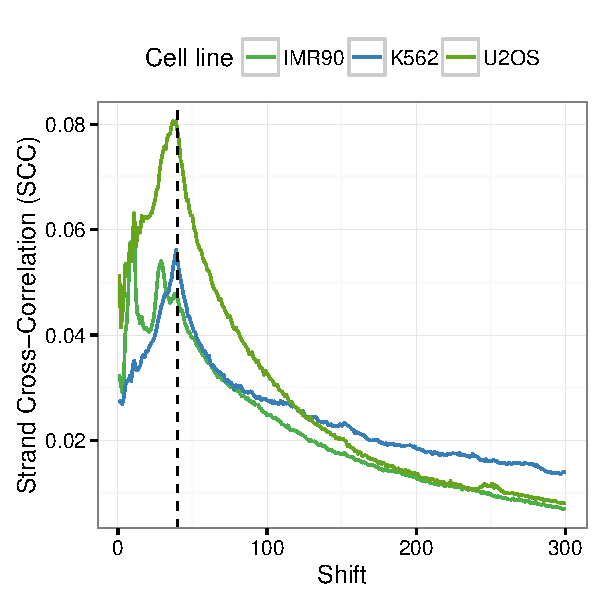
\includegraphics[width =
  .5\textwidth]{figures/supplement/SCC/Meijsing_GR_SCC.pdf}
  \caption{SCC curves for GR factor in IMR90, K562 and U2OS human cell
    lines.}
  \label{sfig:scc3}
\end{figure}

\begin{figure}[H]
  \centering
  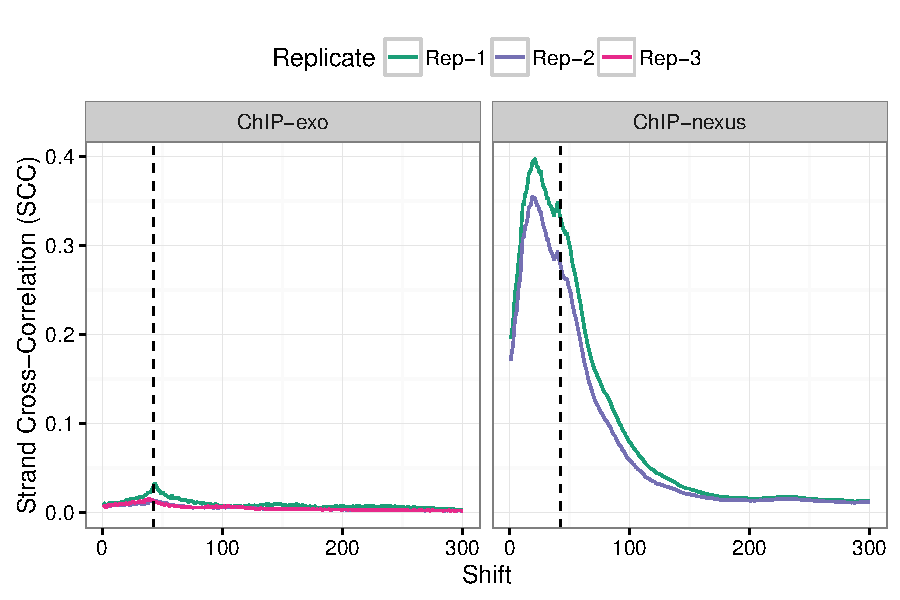
\includegraphics[width =
  .75\textwidth]{figures/supplement/SCC/TBP_K562_SCC.pdf}
  \caption{Comparison of ChIP-exo vs. ChIP-nexus SCC curves for TBP
    factor in human K562 cell lines.}
  \label{sfig:scc4}
\end{figure}

\begin{figure}[H]
  \centering
  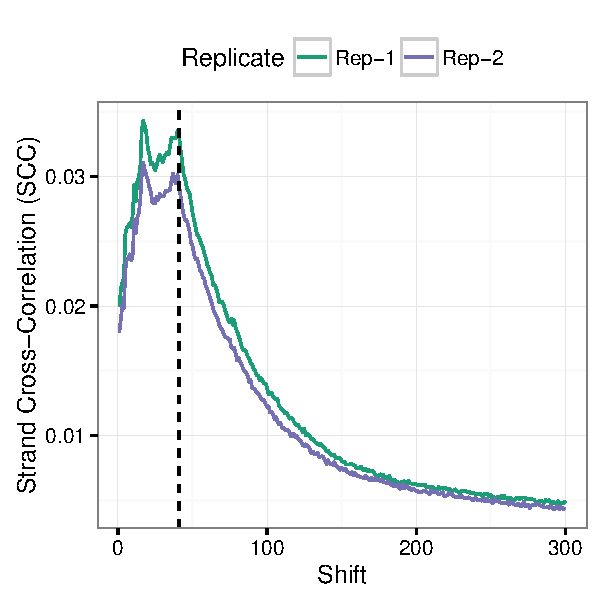
\includegraphics[width =        
  .5\textwidth]{figures/supplement/SCC/Nexus_embryo_dorsal_SCC.pdf}
  \caption{SCC curves for dorsal factor in embryo
    \emph{D. Melanogaster} cell lines.}
  \label{sfig:scc5}
\end{figure}

\begin{figure}[H]
  \centering
  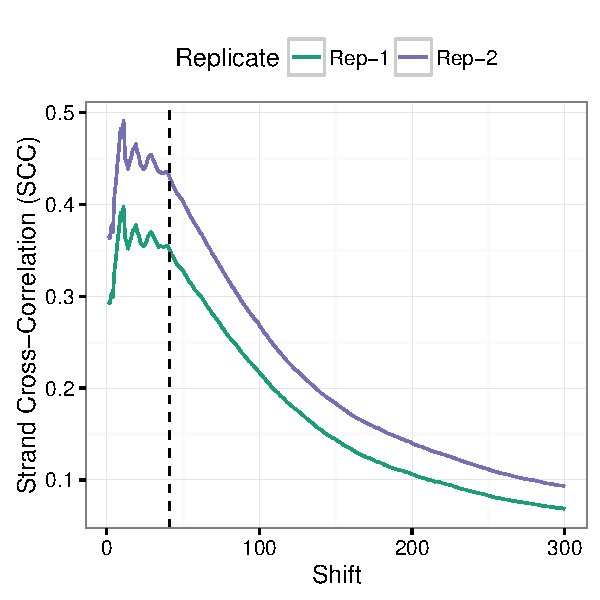
\includegraphics[width =
  .5\textwidth]{figures/supplement/SCC/Nexus_embryo_twist_SCC.pdf}
  \caption{SCC curves for twist factor in embryo
    \emph{D. Melanogaster} cell lines.}
  \label{sfig:scc6}
\end{figure}

\begin{figure}[H]
  \centering
  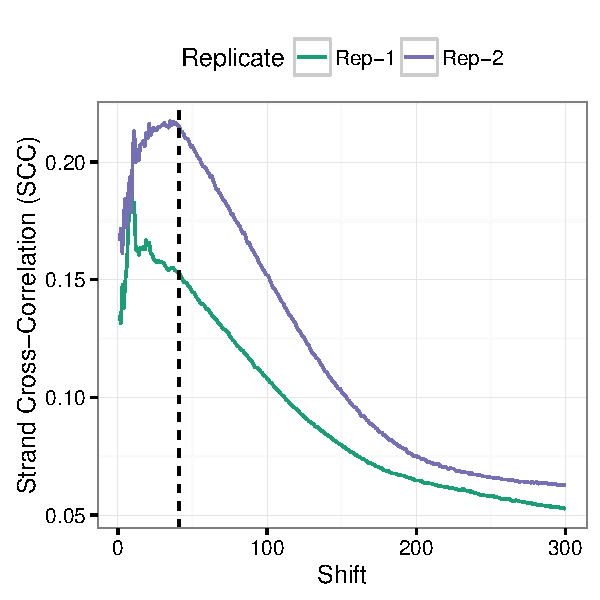
\includegraphics[width =
  .5\textwidth]{figures/supplement/SCC/Nexus_S2_Max_SCC.pdf}
  \caption{SCC curves for Max factor in S2 \emph{D. Melanogaster} cell
    lines.}
  \label{sfig:scc7}
\end{figure}

\begin{figure}[H]
  \centering
  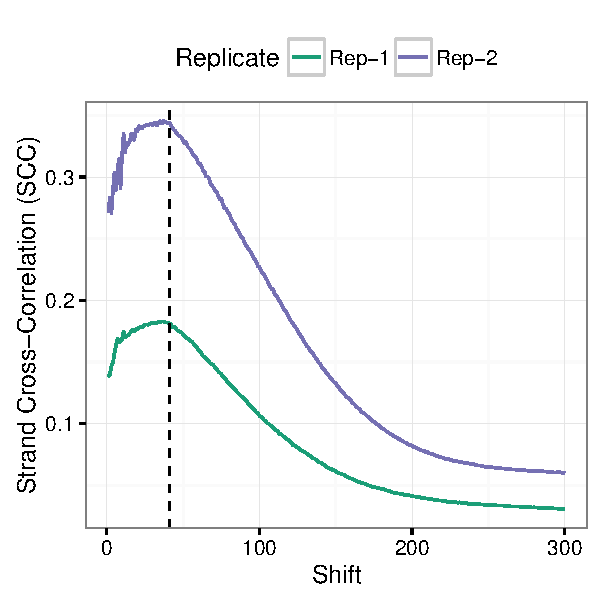
\includegraphics[width =
  .5\textwidth]{figures/supplement/SCC/Nexus_S2_MyC_SCC.pdf}
  \caption{SCC curves for MyC factor in S2 \emph{D. Melanogaster} cell
    lines.}
  \label{sfig:scc8}
\end{figure}

\RW{need to generate this curves for sig70 samples, compared against
  PE and SE ChIP-seq}

\newpage

\section{QC pipeline applied to ChIP-exo and ChIP-nexus data.}

\begin{figure}[H]
  \centering
  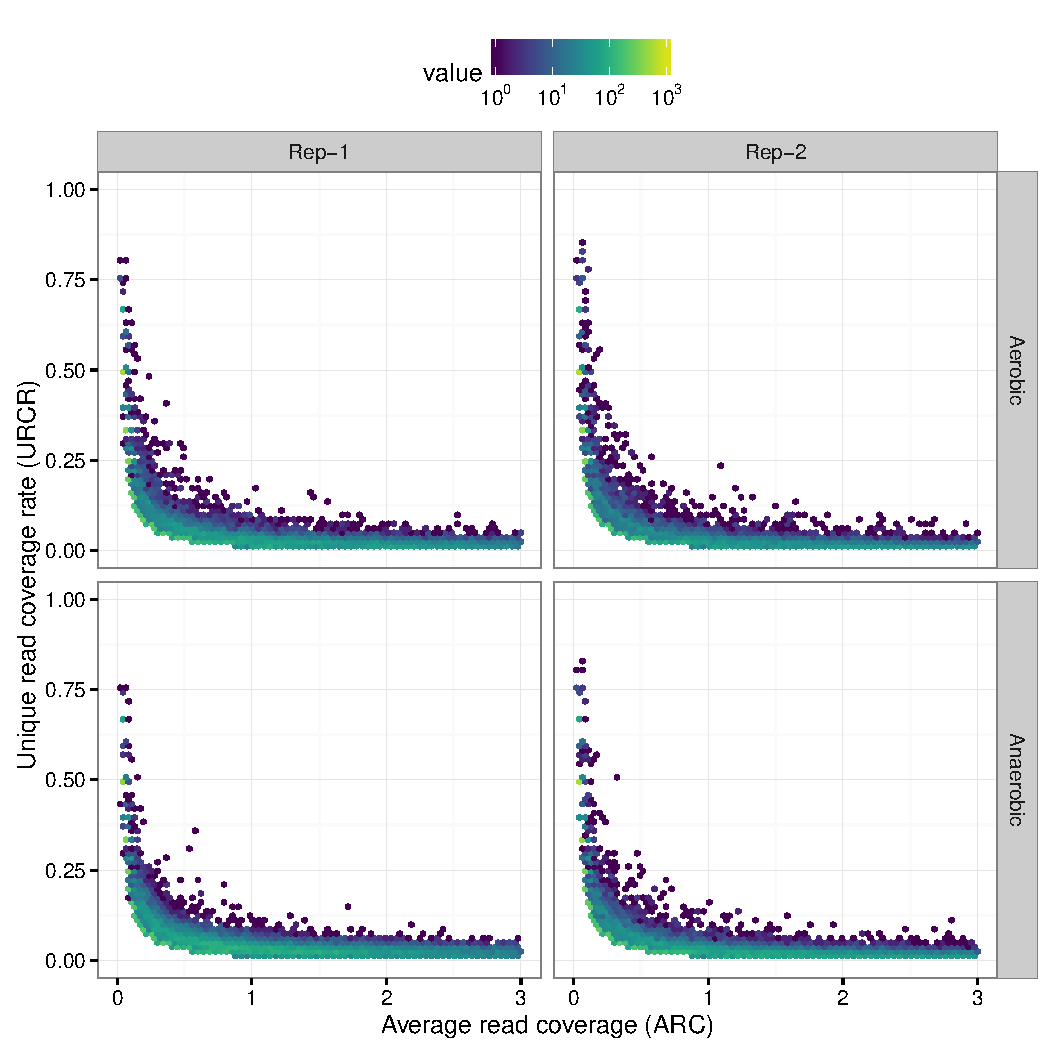
\includegraphics[width = .5\textwidth,page =
1]{figures/supplement/QC/Sig70_bios1_enrichment.pdf}\\
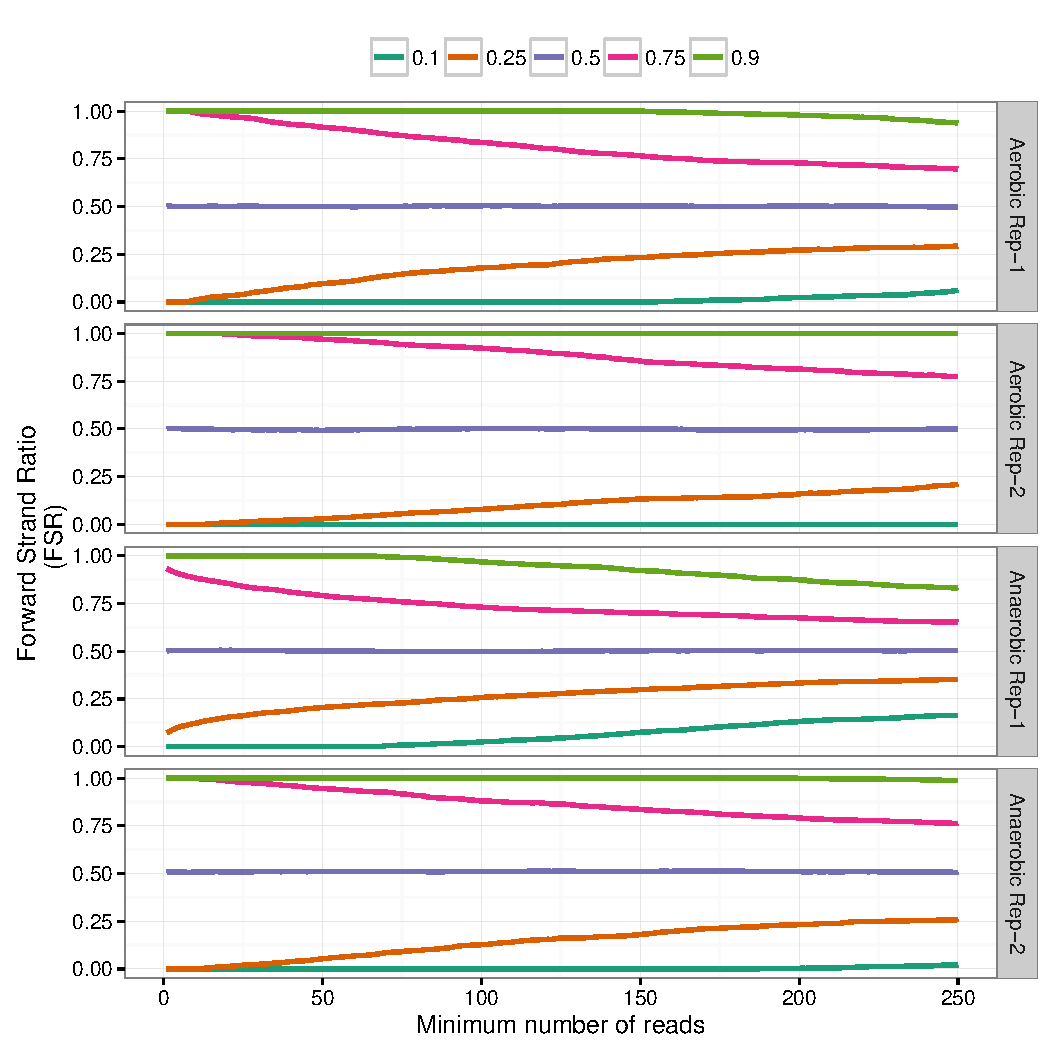
\includegraphics[width = .45\textwidth,page =
1]{figures/supplement/QC/Sig70_bios1_strand_imbalance.pdf}
\includegraphics[width = .45\textwidth,page =
3]{figures/supplement/QC/Sig70_bios1_strand_imbalance.pdf}
\caption{ChIP-exo QC pipeline diagnostics for $\sigma^{70}$ E1
  biosample in \emph{E. Coli}.}
  \label{sfig:qc1}
\end{figure}

\begin{figure}[H]
  \centering
  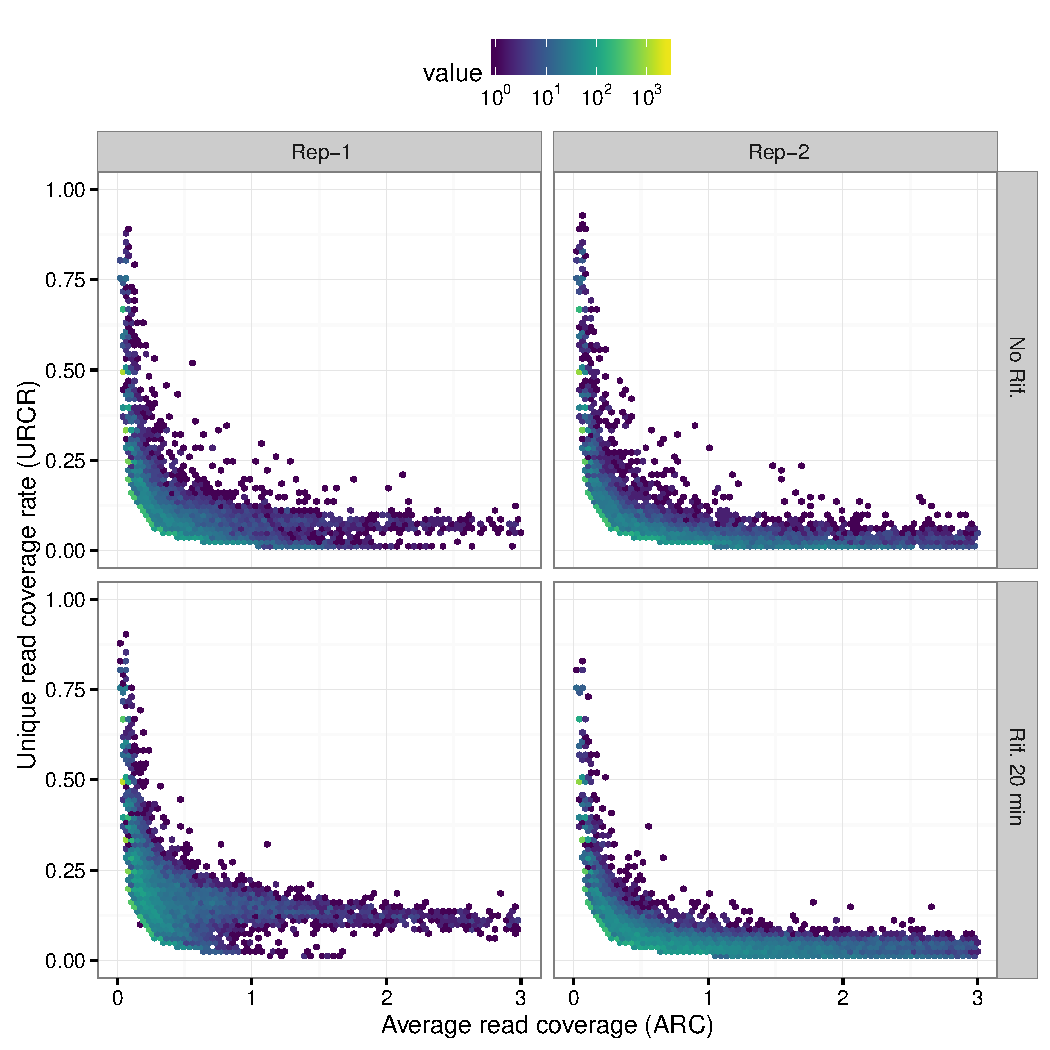
\includegraphics[width = .5\textwidth,page =
1]{figures/supplement/QC/Sig70_bios2_enrichment.pdf}\\
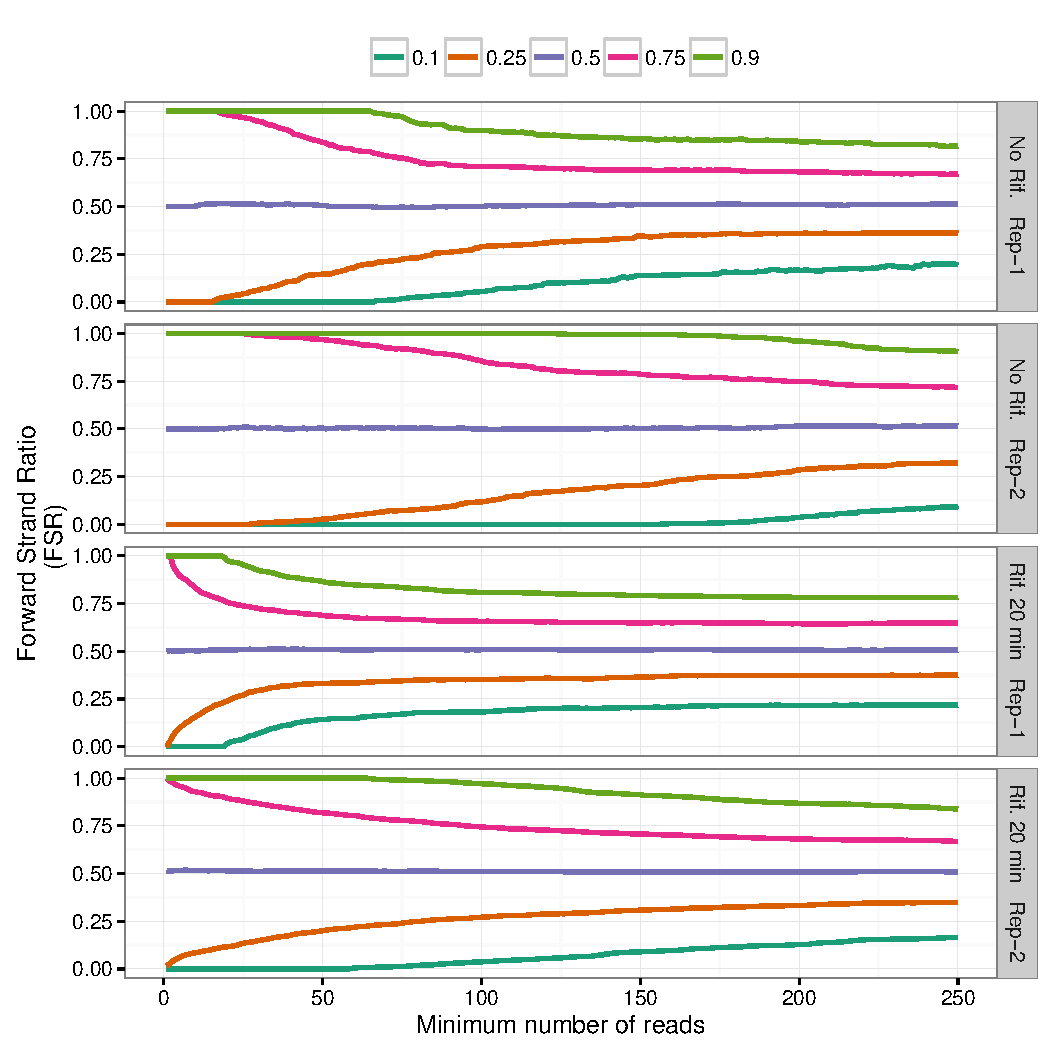
\includegraphics[width = .45\textwidth,page =
1]{figures/supplement/QC/Sig70_bios2_strand_imbalance.pdf}
\includegraphics[width = .45\textwidth,page =
3]{figures/supplement/QC/Sig70_bios2_strand_imbalance.pdf}
\caption{ChIP-exo QC pipeline diagnostics for $\sigma^{70}$ E2
  biosample in \emph{E. Coli}.}
  \label{sfig:qc2}
\end{figure}

\begin{figure}[H]
  \centering
  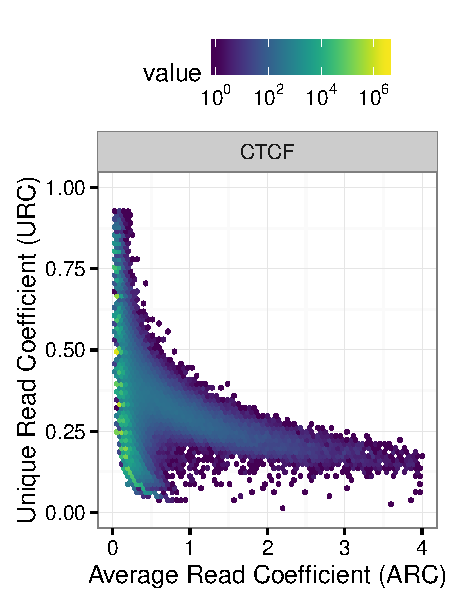
\includegraphics[width = .35\textwidth,page =
1]{figures/supplement/QC/Pugh_CTCF_hela_enrichment.pdf}\\
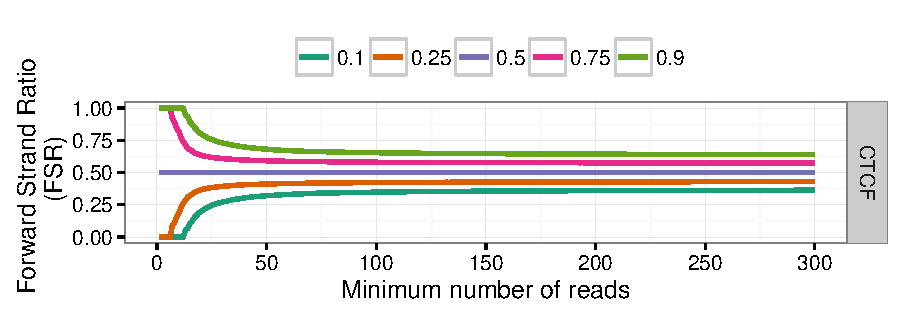
\includegraphics[width = .65\textwidth,page =
1]{figures/supplement/QC/Pugh_CTCF_hela_strand_imbalance.pdf}
\includegraphics[width = .65\textwidth,page =
3]{figures/supplement/QC/Pugh_CTCF_hela_strand_imbalance.pdf}
\caption{ChIP-exo QC pipeline diagnostics for CTCF factor in human
  HeLa cell lines.}
  \label{sfig:qc3}
\end{figure}

\begin{figure}[H]
  \centering
  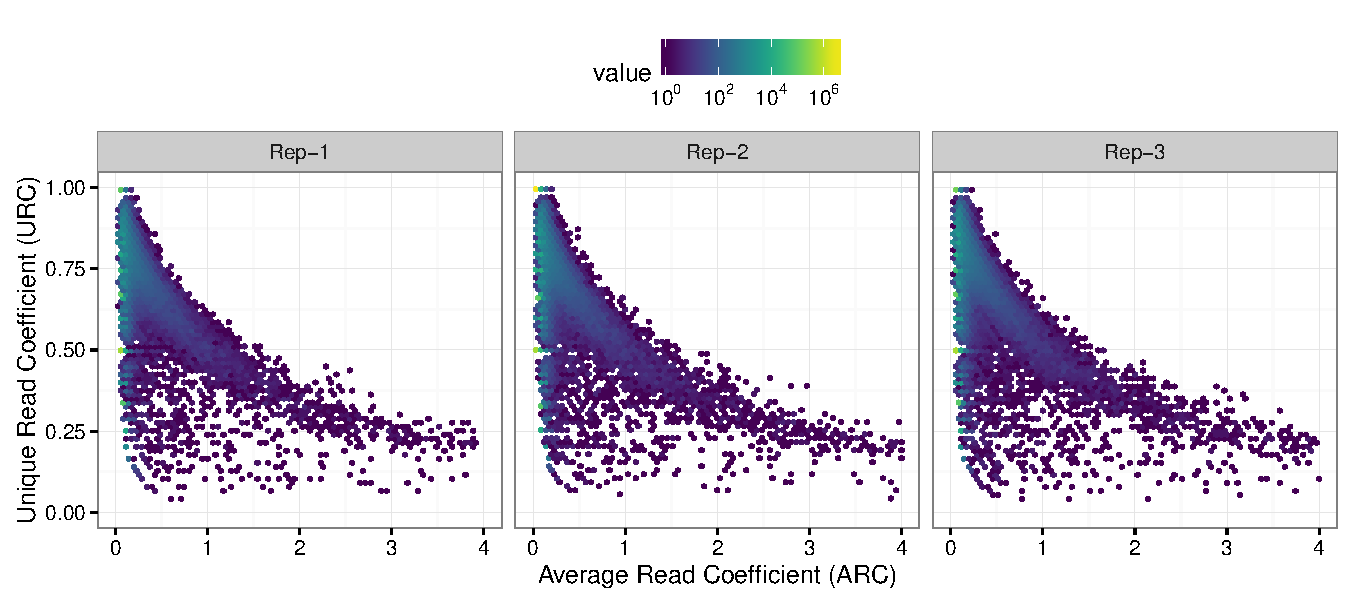
\includegraphics[width = .75\textwidth,page =
1]{figures/supplement/QC/Carroll_ER_MCF7_enrichment.pdf}\\
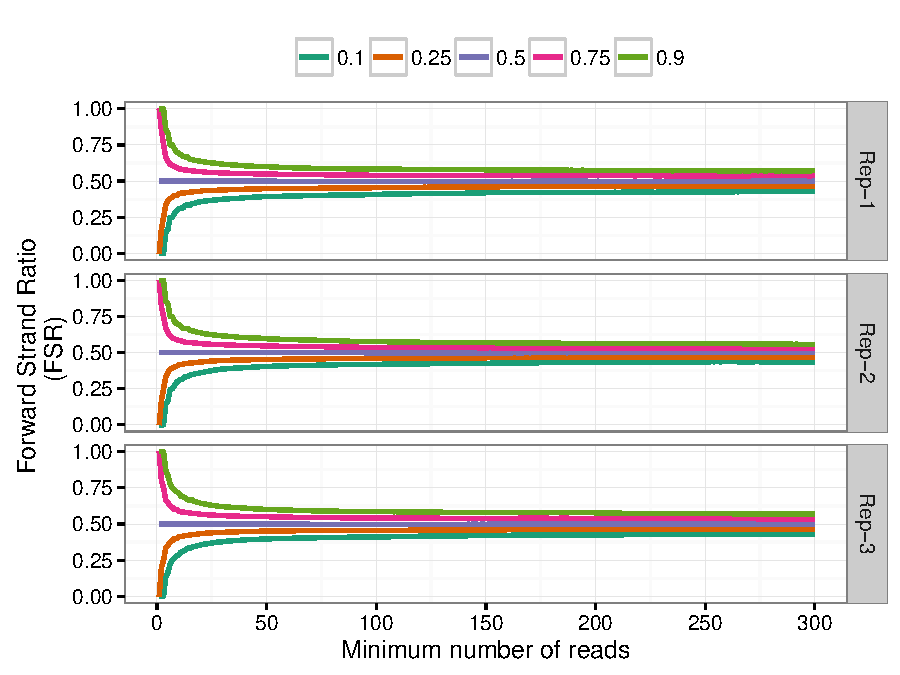
\includegraphics[width = .65\textwidth,page =
1]{figures/supplement/QC/Carroll_ER_MCF7_strand_imbalance.pdf}
\includegraphics[width = .65\textwidth,page =
3]{figures/supplement/QC/Carroll_ER_MCF7_strand_imbalance.pdf}
  \caption{ChIP-exo QC pipeline diagnostics for ER factor in human MCF-7 cell lines.}
  \label{sfig:qc4}
\end{figure}

\begin{figure}[H]
  \centering
  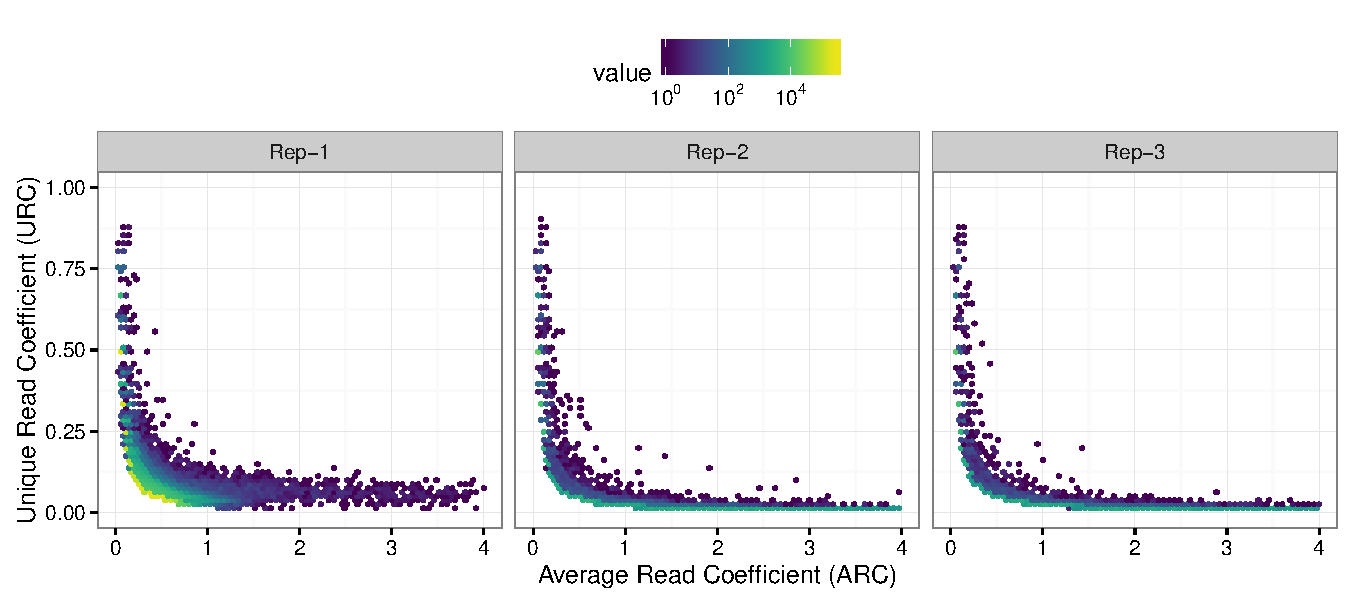
\includegraphics[width = .75\textwidth,page =
1]{figures/supplement/QC/Venters_K562_TBP_enrichment.pdf}\\
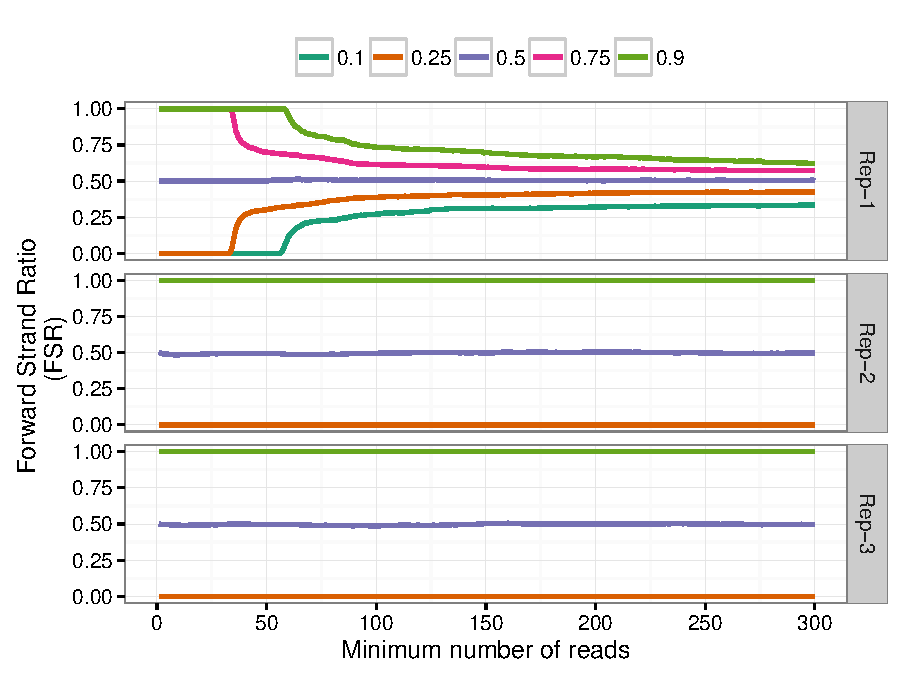
\includegraphics[width = .65\textwidth,page =
1]{figures/supplement/QC/Venters_K562_TBP_strand_imbalance.pdf}
\includegraphics[width = .65\textwidth,page =
3]{figures/supplement/QC/Venters_K562_TBP_strand_imbalance.pdf}
\caption{ChIP-exo QC pipeline diagnostics for TBP factor in human K562
  cell lines.}
  \label{sfig:qc5}
\end{figure}

\begin{figure}[H]
  \centering
  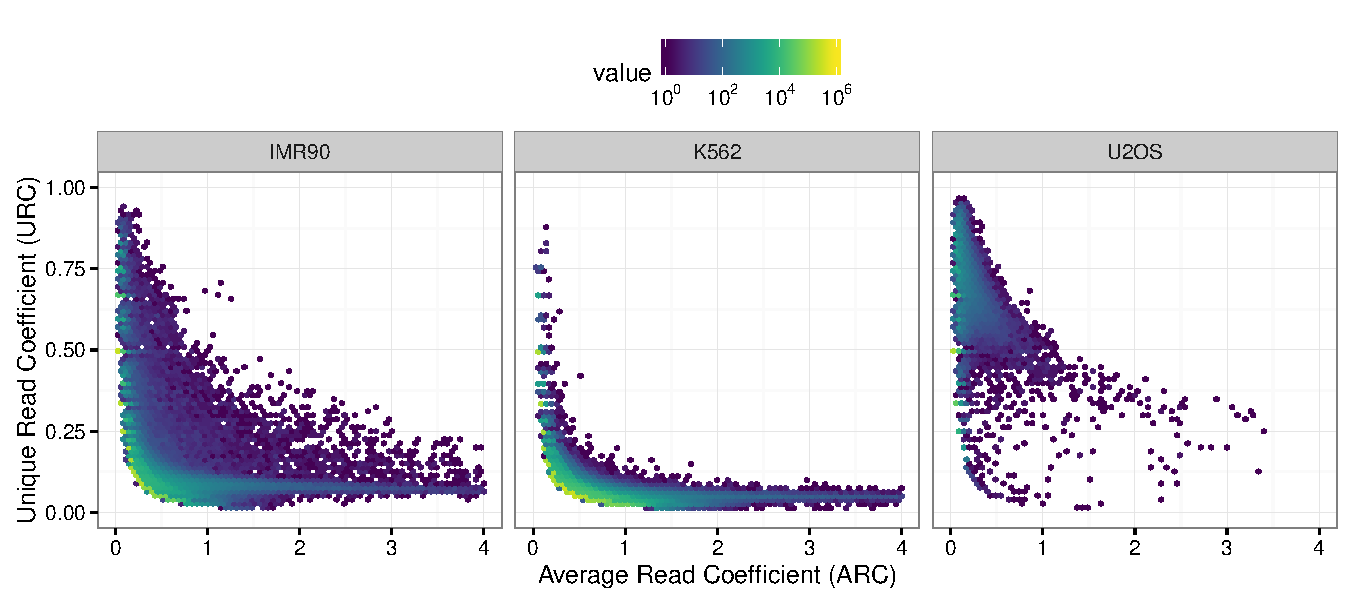
\includegraphics[width = .75\textwidth,page =
1]{figures/supplement/QC/Meijsing_GR_enrichment.pdf}\\
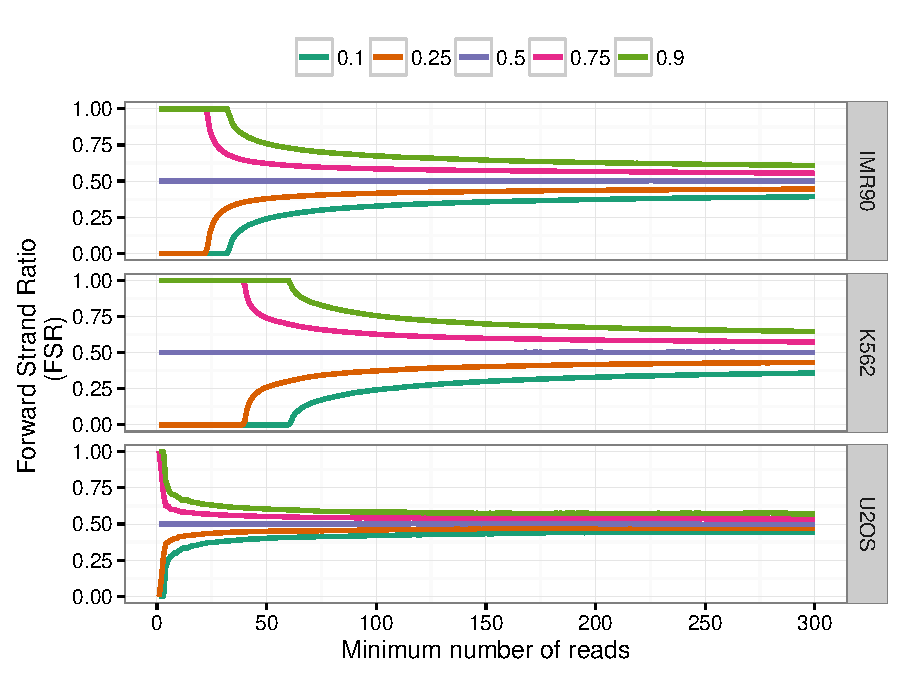
\includegraphics[width = .65\textwidth,page =
1]{figures/supplement/QC/Meijsing_GR_strand_imbalance.pdf}
\includegraphics[width = .65\textwidth,page =
3]{figures/supplement/QC/Meijsing_GR_strand_imbalance.pdf}
\caption{ChIP-exo QC pipeline diagnostics for GR factor in human
  IMR90, K562 and U2OS cell lines respectively.}
  \label{sfig:qc6}
\end{figure}


\begin{figure}[H]
  \centering
  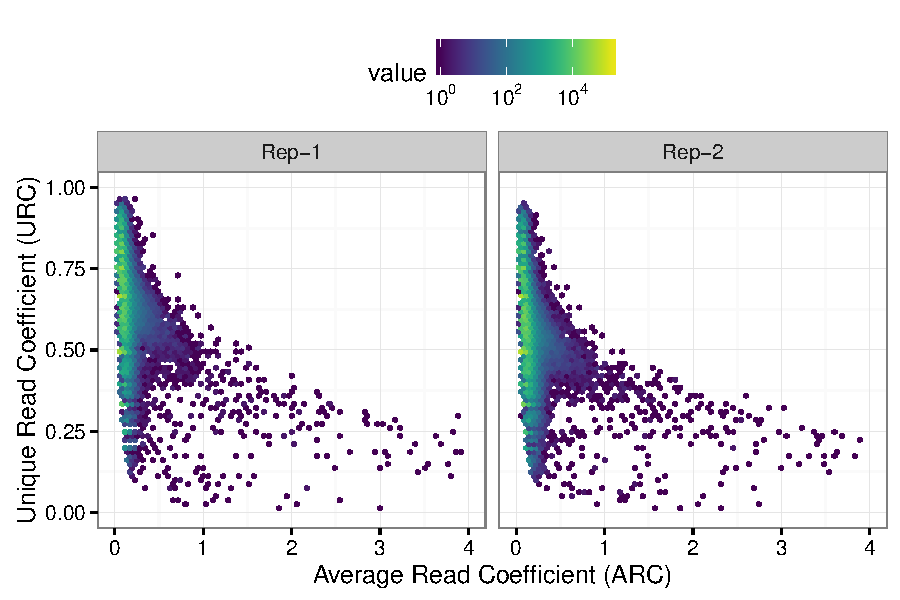
\includegraphics[width = .65\textwidth,page =
1]{figures/supplement/QC/ChIPnexus_embryo_dorsal_enrichment.pdf}\\
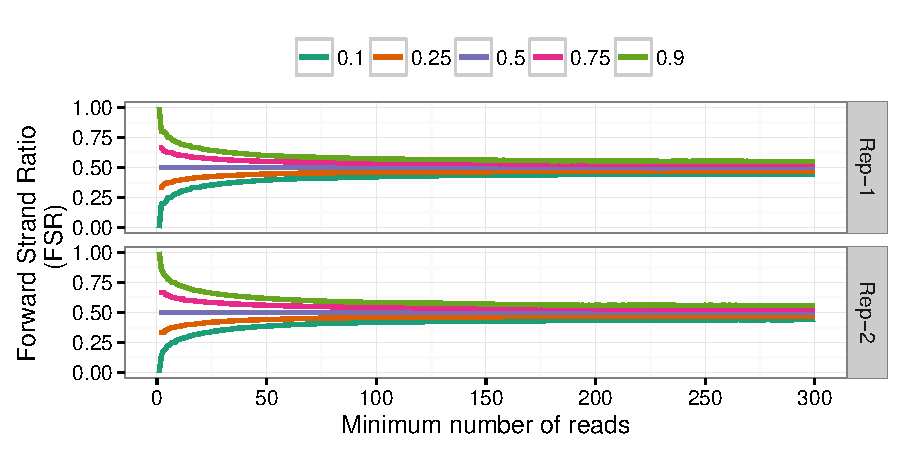
\includegraphics[width = .65\textwidth,page =
1]{figures/supplement/QC/ChIPnexus_embryo_dorsal_strand_imbalance.pdf}
\includegraphics[width = .65\textwidth,page =
3]{figures/supplement/QC/ChIPnexus_embryo_dorsal_strand_imbalance.pdf}
\caption{ChIP-exo QC pipeline diagnostics for ChIP-nexus experiment of
  dorsal factor in embryo \emph{D. Melanogaster} cell lines.}
  \label{sfig:qc7}
\end{figure}

\begin{figure}[H]
  \centering
  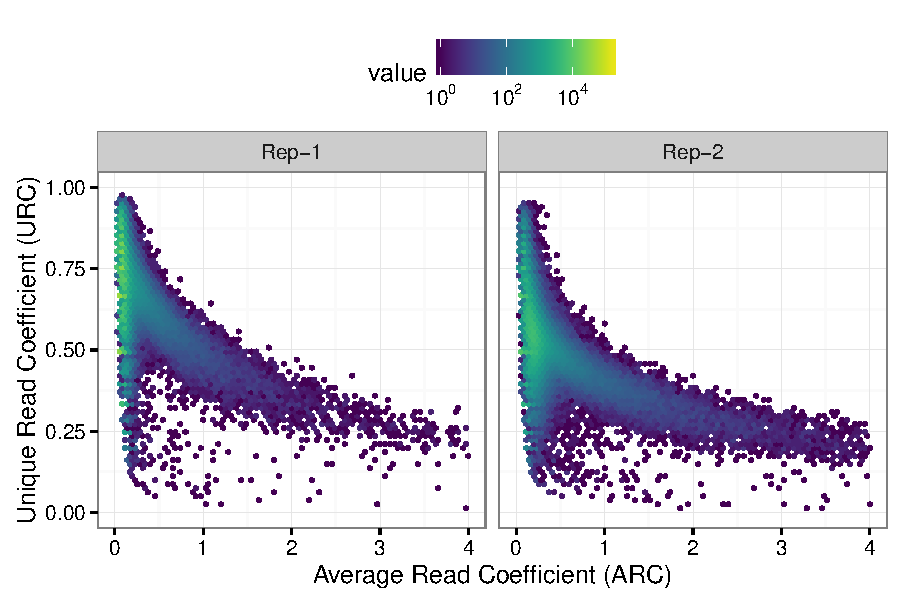
\includegraphics[width = .65\textwidth,page =
1]{figures/supplement/QC/ChIPnexus_embryo_twist_enrichment.pdf}\\
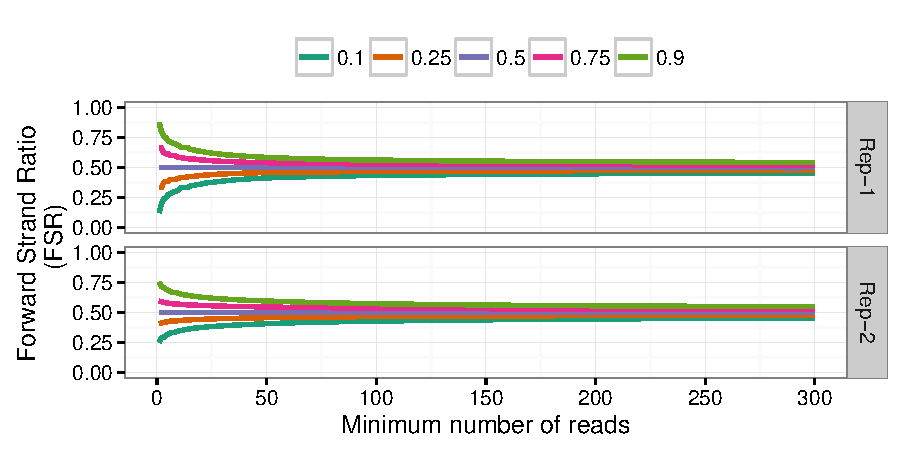
\includegraphics[width = .65\textwidth,page =
1]{figures/supplement/QC/ChIPnexus_embryo_twist_strand_imbalance.pdf}
\includegraphics[width = .65\textwidth,page =
3]{figures/supplement/QC/ChIPnexus_embryo_twist_strand_imbalance.pdf}
\caption{ChIP-exo QC pipeline diagnostics for ChIP-nexus experiment of
  twist factor in embryo \emph{D. Melanogaster} cell lines.}
  \label{sfig:qc8}
\end{figure}

\begin{figure}[H]
  \centering
  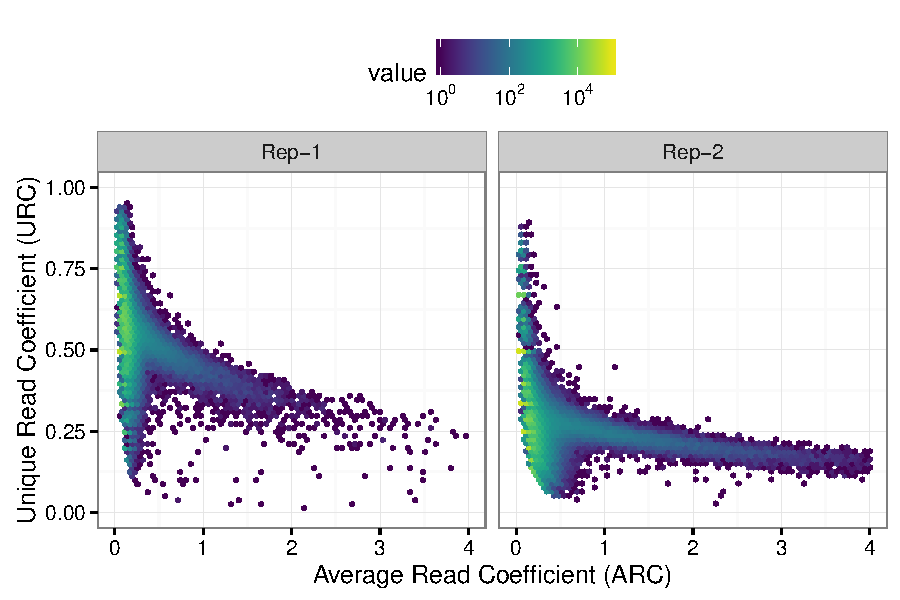
\includegraphics[width = .65\textwidth,page =
1]{figures/supplement/QC/ChIPnexus_S2_max_enrichment.pdf}\\
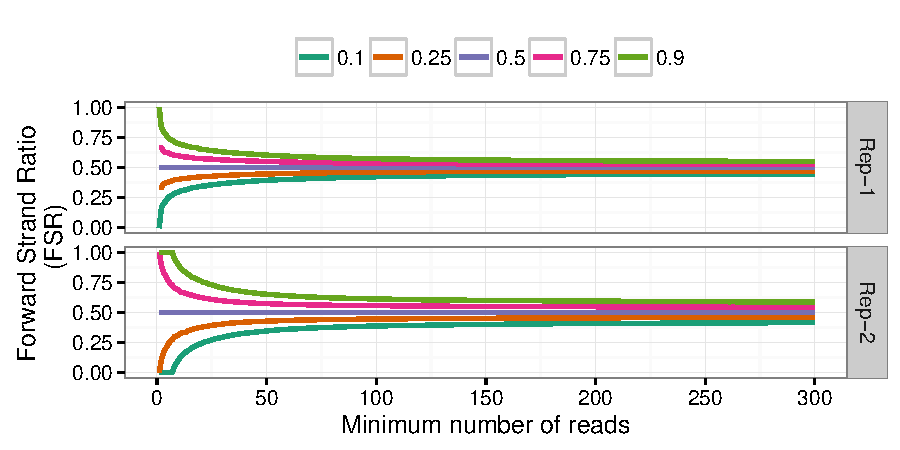
\includegraphics[width = .65\textwidth,page =
1]{figures/supplement/QC/ChIPnexus_S2_max_strand_imbalance.pdf}
\includegraphics[width = .65\textwidth,page =
3]{figures/supplement/QC/ChIPnexus_S2_max_strand_imbalance.pdf}
\caption{ChIP-exo QC pipeline diagnostics for ChIP-nexus experiment of
  Max factor in S2 \emph{D. Melanogaster} cell lines.}
  \label{sfig:qc9}
\end{figure}

\begin{figure}[H]
  \centering
  \includegraphics[width = .65\textwidth,page =
1]{figures/supplement/QC/ChIPnexus_S2_myc_enrichment.pdf}\\
\includegraphics[width = .65\textwidth,page =
1]{figures/supplement/QC/ChIPnexus_S2_myc_strand_imbalance.pdf}
\includegraphics[width = .65\textwidth,page =
3]{figures/supplement/QC/ChIPnexus_S2_myc_strand_imbalance.pdf}
\caption{ChIP-exo QC pipeline diagnostics for ChIP-nexus experiment of
  MyC factor in S2 \emph{D. Melanogaster} cell lines.}
  \label{sfig:qc10}
\end{figure}


\begin{figure}[H]
  \centering
  \includegraphics[width = .65\textwidth,page =
1]{figures/supplement/QC/ChIPnexus_K562_TBP_enrichment.pdf}\\
\includegraphics[width = .65\textwidth,page =
1]{figures/supplement/QC/ChIPnexus_K562_TBP_strand_imbalance.pdf}
\includegraphics[width = .65\textwidth,page =
3]{figures/supplement/QC/ChIPnexus_K562_TBP_strand_imbalance.pdf}
\caption{ChIP-exo QC pipeline diagnostics for ChIP-nexus experiment of
  TBP factor in K562 human cell lines.}
  \label{sfig:qc11}
\end{figure}

\newpage

\subsection*{Comparison of QC pipeline for different sub-sampled
  sequencing depths.}

\begin{figure}[H]
  \centering
  \includegraphics[width =.95\textheight,angle = 90,page =
1]{figures/supplement/QC_samp/Sig70_sample_bios1_enrichment.pdf} 
\end{figure}

\begin{figure}[H]
  \centering
  \includegraphics[width =.9\textheight,angle = 90,page =
1]{figures/supplement/QC_samp/Sig70_sample_bios1_strand_imbalance.pdf} 
\end{figure}

\begin{figure}[H]
  \centering
  \includegraphics[width =.9\textheight,angle = 90,page =
3]{figures/supplement/QC_samp/Sig70_sample_bios1_strand_imbalance.pdf} 
  \label{sfig:qcsamp1}
  \caption{ChIP-exo QC pipeline diagnostics for $\sigma^{70}$ E1
    biosample on \emph{E. Coli} when sampling 10K to 100K reads from
    each experiment}
\end{figure}

\begin{figure}[H]
  \centering
  \includegraphics[width =.95\textheight,angle = 90,page =
1]{figures/supplement/QC_samp/Sig70_sample_bios2_enrichment.pdf} 
\end{figure}

\begin{figure}[H]
  \centering
  \includegraphics[width =.9\textheight,angle = 90,page =
1]{figures/supplement/QC_samp/Sig70_sample_bios2_strand_imbalance.pdf} 
\end{figure}

\begin{figure}[H]
  \centering
  \includegraphics[width =.9\textheight,angle = 90,page =
3]{figures/supplement/QC_samp/Sig70_sample_bios2_strand_imbalance.pdf} 
  \caption{ChIP-exo QC pipeline diagnostics for $\sigma^{70}$ E2
    biosample on \emph{E. Coli} when sampling 10K to 100K reads from
    each experiment}
  \label{sfig:qcsamp2}
\end{figure}

\begin{figure}[H]
  \centering
  \includegraphics[height = .4\textheight,page =
  1]{figures/supplement/QC_samp/TBP_sample_enrichment.pdf}
  \includegraphics[height = .25\textheight,page =
1]{figures/supplement/QC_samp/TBP_sample_strand_imbalance.pdf} 
  \includegraphics[height = .25\textheight,page =
3]{figures/supplement/QC_samp/TBP_sample_strand_imbalance.pdf} 
\caption{ChIP-exo QC pipeline diagnostics applied to ChIP-nexus and
  ChIP-exo experiments of TBP factor in K562 human cell lines when
  sampling 20M to 50M reads from each experiment.}
  \label{sfig:qcsamp3}
\end{figure}



\newpage

\subsection{FoxA1 peak overlaps with high quality regions.}

\begin{figure}[H]
\begin{center}
  \includegraphics[width=.45\textwidth,page =
  1]{figures/supplement/peak_overlaps/FoxA1_VennDiagram_QC_region_w_motif_and_peaks.pdf} \\
\includegraphics[width=.45\textwidth,page =
2]{figures/supplement/peak_overlaps/FoxA1_VennDiagram_QC_region_w_motif_and_peaks.pdf}\\
\includegraphics[width=.45\textwidth,page =
3]{figures/supplement/peak_overlaps/FoxA1_VennDiagram_QC_region_w_motif_and_peaks.pdf}\\
\end{center}
\caption{Venn diagrams of high quality regions that overlap peaks for
  FoxA1 factor in mouse liver cell lines. Top) Rep-1, Middle) Rep-2
  and Bottom) Rep-3.}
\label{sfig:venn}
\end{figure}

\newpage

% \subsection{Evaluation of sub-sampled experiment with QC pipeline.}

% \newpage


% \section{Comparison with other methods rif samples.}

% \newpage


% \section{Saturation analysis rif samples.} %% need to re -do


% \newpage

% \section{Resolution and sensitivity.}

\end{document}
